
\chapter{Aplikace v konkrétních rodinách distribucí}

V této kapitole použijeme minimální Rényiho odhady ($\mathfrak{R}_\alpha$-odhady) pro konkrétní rozdělení pravděpodobnosti. Výsledky pro normální model byly uvedeny již v \cite{Vajda2009}, \cite{Demut2010}, my jsme se tedy zaměřili na exponenciální, Laplaceovo, Cauchyho a Weibullovo rozdělení. V případě těchto rodin jsme se snažili o odvození konkrétního tvaru odhadu podle \eqref{Renyi-estimator_formula} a také tvaru influeční funkce \eqref{IF}.

\section{Laplaceovo rozdělení} %%%%%%%%%%%%%%%%%%%%%  LAPLACE   %%%%%%%%%%%%%%%%%%%%%%

Zde použijeme minimální $\mathfrak{R}_\alpha$-odhady k odhadu parametru $\theta = (\mu,\lambda)$ pro Laplaceův model. Hustota pravděpodobnosti má tedy tvar
\begin{equation}
	p_\theta = \frac{1}{2\lambda} e^{-\frac{|x-\mu|}{\lambda}}, \qquad \mu\in \mathbb{R},\, \lambda>0.
\end{equation}
Pro $\alpha = 0$ se odhad podle \eqref{Renyi-estimator_formula} rovná maximálně věrohodnému odhadu
\begin{align}
	\hat{\theta}_{\mathfrak{R}_0,n} & = \arg \max_{\theta \in \Theta} \frac{1}{n} \sum^n_{i=1} \ln \left[ \frac{1}{2\lambda}\exp \left[-\frac{|x_i-\mu|}{\lambda} \right] \right] \nonumber \\
	& =  \arg \max_{\theta \in \Theta} \left[ \ln \frac{1}{2\lambda} - \frac{1}{n} \sum^n_{i=1} \frac{|x_i-\mu|}{\lambda} \right].
\end{align}
Protože podmínka \eqref{beta-podminka} platí pro každé $\beta>0$, můžeme tedy min $\mathfrak{R}_\alpha$-odhad \eqref{Renyi-estimator_formula} parametrů Laplaceova rozdělení psát pro $\alpha>0$ jako 
\begin{equation}
	\hat{\theta}_{\mathfrak{R}_\alpha,n} = \arg \max_{\theta \in \Theta} \left[ (2\lambda)^{-\frac{\alpha}{1+\alpha}} \frac{1}{n} \sum_{i=1}^n \exp \left[-\alpha\frac{|x_i-\mu|}{\lambda} \right] \right].
	\label{renyi-formula-laplace}
\end{equation}

\noindent Vzorec \eqref{renyi-formula-laplace} je pro současný odhad obou parametrů $\mu, \lambda$. Pokud by byl jeden z parametrů známý a nebylo ho tedy nutné odhadovat, dosadíme jeho hodnotu do vzorce a maximalizujeme pak jen v jedné proměnné. 

Nyní pro {\mRao} v Laplaceově modelu spočítáme influenční funkce podle \eqref{IF}. Pro odhad polohy $\theta = \mu$ při známém parametru $\lambda$, dostáváme influenční funkci ve tvaru

\begin{equation}
	\mathrm{IF}(x;T_{\mathfrak{R}_\alpha},\mu) = (1+\alpha )^{\frac{3}{2}} (x-\mu )  e^{-\frac{\alpha}{2} (x-\mu )^2}. % IF(x,mu)
	\label{IF-laplace-mu}
\end{equation}
Pokud prohodíme úlohu parametrů, tedy pokud budeme odhadovat měřítko $\theta = \lambda$, zatímco polohu $ \mu$ budeme považovat za známou, dostaneme 
\begin{equation}
	\mathrm{IF}(x;T_{\mathfrak{R}_\alpha},\lambda) = (1 + \alpha)^2 \left(-\lambda + (1 + \alpha)|x-\mu|\right)  e^{-\frac{\alpha|x-\mu|}{\lambda}}	. % IF(x,sigma)
	\label{IF-laplace-lambda}
\end{equation}

\begin{figure}[htb]
\begin{center}
\begin{tabular}{c c c}
	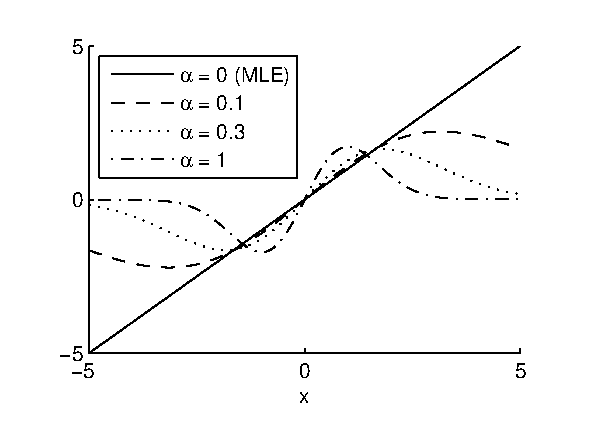
\epsfig{file=Laplace-IF-mu.eps, height=2.in} 
	&&
	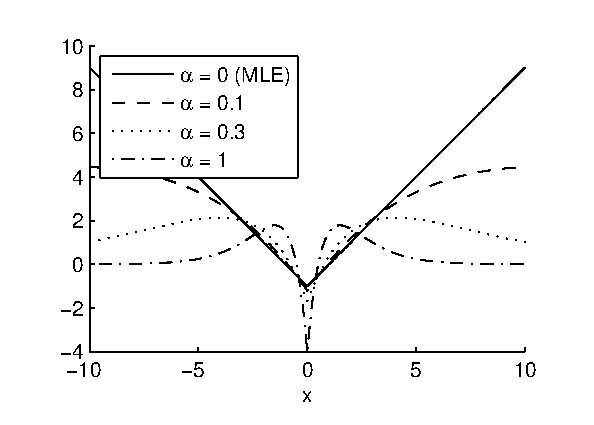
\epsfig{file=Laplace-IF-lambda.eps, height=2.in} 
	\\
	$\mathrm{IF}(x;T_{\mathfrak{R}_\alpha},\mu = 0) $ při známém $\lambda = 1$ 
	&&
	$\mathrm{IF}(x;T_{\mathfrak{R}_\alpha},\lambda = 1)$ při známém $\mu = 0$ 
	\\
\end{tabular}
\caption{Influenční funkce minimálních $\mathfrak{R}_\alpha$-odhadů parametrů Laplaceova rozdělení}
\label{fig:laplace-if}
\end{center}
%\label{fig:laplace-if}
\end{figure}

\noindent Z \eqref{IF-laplace-mu} a \eqref{IF-laplace-lambda} vidíme, že jsou obě influenční funkce pro $\alpha>0$ omezené, tedy B-robustní a navíc pro obě funkce platí

\begin{equation}
	\lim_{x \rightarrow \pm\infty} \mathrm{IF}(x;T_{\mathfrak{R}_\alpha},\cdot) = 0.
\end{equation}
 
\noindent Nemáme sice konečný bod zamítání $\rho^*$, ale influenční funkce se alespoň limitně blíží s rostoucím $x$ k nule. Tato konvergence je s větším $\alpha$ rychlejší kvůli členu $e^{-\alpha x}$, který se vyskytuje v obou funkcích. To je vidět i na obrázku \ref{fig:laplace-if}, kde jsou vyobrazeny influenční funkce zvlášť pro oba odhadované parametry a s různými hodnotami $\alpha$. Je vidět, že maximálně věrohodný odhad $(\alpha = 0)$ není omezený, a že se funkce pro větší hodnoty $\alpha$ s rostoucí vzdáleností hodnot $x$ od polohy $\mu=0$ rychleji blíží k nule.

\section{Exponenciální rozdělení} %%%%%%%%%%%%%%%%%%%%%  EXPONENTIAL   %%%%%%%%%%%%%%%%%%%%%%

Nyní použijeme minimální $\mathfrak{R}_\alpha$-odhady k odhadu parametru $\theta = (\mu,\lambda)$ pro případ exponenciálního rozdělení s hustotou pravděpodobnosti
\begin{equation}
	p_\theta = \frac{1}{\lambda} e^{-\frac{x-\mu}{\lambda}}, \qquad \mu\in \mathbb{R},\, \lambda>0, \, x\geq\mu.
\end{equation}
\noindent Exponenciální hustota je svým tvarem velmi podobná té Laplaceově. Dále uvidíme, že i vzorce týkající se minimálních Rényiho odhadů vycházejí pro oba modely velmi podobně, v některých případech dokonce stejně.  Pro $\alpha = 0$ dostáváme odhad ve tvaru
\begin{align}
	\hat{\theta}_{\mathfrak{R}_0,n} & =  \arg \max_{\theta \in \Theta} \frac{1}{n} \sum^n_{i=1} \ln \left[ \frac{1}{\lambda}\exp \left[-\frac{x_i-\mu}{\lambda} \right] \right] \nonumber \\
	& =  \arg \max_{\theta \in \Theta} \left[ \ln \frac{1}{\lambda} - \frac{1}{n} \sum^n_{i=1} \frac{x_i-\mu}{\lambda} \right].
\end{align}

\noindent Podmínka \ref{beta-podminka} opět platí pro každé $\beta>0$, minimální Rényiho odhad pro $\alpha>0$ můžeme tedy pro exponenciální rodinu psát ve tvaru

\begin{equation}
	\hat{\theta}_{\mathfrak{R}_\alpha,n} = \arg \max_{\theta \in \Theta} \lambda^{-\frac{\alpha}{1+\alpha}} \frac{1}{n}\sum_{i=1}^n \exp \left[-\alpha\frac{x_i-\mu}{\lambda} \right].
	\label{renyi-formula-exponential}
\end{equation}

\noindent Je vidět, že rozdíl oproti \eqref{renyi-formula-laplace} je jen v použití absolutní hodnoty v odhadu Laplaceova modelu. 

Influenční funkce je podle $\eqref{IF}$ v případě odhadu parametru polohy $\theta = \mu$ a známého měřítka $ \lambda$ stejná jako pro Laplaceovo rozdělení $\eqref{IF-laplace-mu}$, tedy 

\begin{equation}
	\mathrm{IF}(x;T_{\mathfrak{R}_\alpha},\mu) = (1+\alpha )^{\frac{3}{2}} (x-\mu )  e^{-\frac{\alpha}{2} (x-\mu )^2}. % IF(x,mu)
	\label{IF-exponential-mu}
\end{equation}
Pokud odhadujeme parametr měřítka $\theta = \lambda$ při známé poloze $ \mu $, vychází funkce ve tvaru
\begin{equation}
	\mathrm{IF}(x;T_{\mathfrak{R}_\alpha},\lambda) =	(1+\alpha )^2 \left( - \lambda +(1+ \alpha)(x-\mu)\right) e^{-\frac{\alpha (x-\mu)}{\lambda }}. % IF(x,lambda),
	\label{IF-exponential-lambda}
\end{equation}

\begin{figure}[htb]
\begin{center}
\begin{tabular}{c c c}
	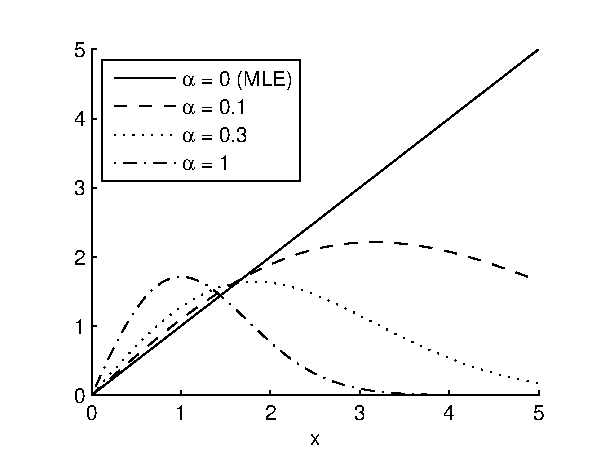
\epsfig{file=Exp-IF-mu.eps, height=2.1in} 
	&&
	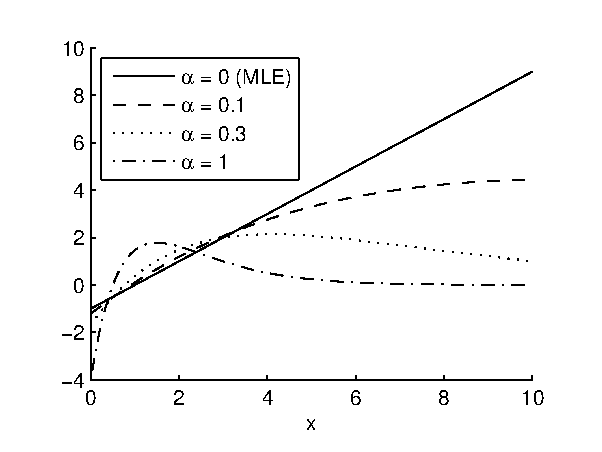
\epsfig{file=Exp-IF-lambda.eps, height=2.1in} 
	\\
	$\mathrm{IF}(x;T_{\mathfrak{R}_\alpha},\mu = 0) $ při známém $\lambda = 1$
	&&
	$\mathrm{IF}(x;T_{\mathfrak{R}_\alpha},\lambda = 1)$ při známém $\mu = 0$
	\\
\end{tabular}
\caption{Influenční funkce minimálních $\mathfrak{R}_\alpha$-odhadů parametrů exponenciálního rozdělení}
\label{fig-exp-if}
\end{center}
\end{figure}

\noindent Ze vzorců \eqref{IF-exponential-mu} a \eqref{IF-exponential-lambda} vidíme, že pro obě funkce platí

\begin{equation}
	\lim_{x \rightarrow \pm\infty} \mathrm{IF}(x;T_{\mathfrak{R}_\alpha},\cdot) = 0,
\end{equation}
tedy že velké outliery budou díky konvergenci influenčních funkcí k nule částečně ignorovány.  Přitom platí, že se konvergence zrychluje s rostoucím $\alpha$, což je vidět na Obr. \ref{fig-exp-if}, stejně jako to, že jsou funkce pro $\alpha >0$ omezené. 

\section{Cauchyovo rozdělení} %%%%%%%%%%%%%%%%%%%%%  Cauchy   %%%%%%%%%%%%%%%%%%%%%%


Dalším rozdělením, na které jsme použili Rényiho odhady, je Cauchyho s parametrem $\theta = (\mu,\sigma)$ a hustotou pravděpodobnosti
\begin{equation}
	p_\theta = \frac{1}{\pi\sigma} \left( 1 + \left( \frac{x-\mu}{\sigma} \right)^2 \right)^{-1}, \qquad \mu\in \mathbb{R},\, \sigma>0.
\end{equation}
Minimální $\mathfrak{R}_\alpha$-odhad je pro $\alpha=0$ roven
\begin{align}
	\hat{\theta}_{\mathfrak{R}_0,n} & = \arg \max_{\theta \in \Theta} \frac{1}{n} \sum^n_{i=1} \ln \left[  \frac{1}{\pi\sigma} \left( 1 + \left( \frac{x_i-\mu}{\sigma} \right)^2 \right)^{-1}   \right] \nonumber \\
	& =  \arg \max_{\theta \in \Theta} \left[ -\ln \pi\sigma - \frac{1}{n} \sum^n_{i=1} \ln \left[ 1 + \left( \frac{x_i-\mu}{\sigma} \right)^2 \right] \right],
\end{align}
který je shodný s maximálně věrohodným odhadem. Podmínka \eqref{beta-podminka} platí tak jako v předchozích případech pro každé $\beta>0$. Pro $\alpha>0$ pak vychází minimální $\mathfrak{R}_\alpha$-odhad \eqref{Renyi-estimator_formula} parametrů v Cauchyho modelu jako 

\begin{equation}
	\hat{\theta}_{\mathfrak{R}_\alpha,n} = \arg \max_{\theta \in \Theta} \left[ \sigma^{-\frac{\alpha}{1+\alpha}} \frac{1}{n} \sum_{i=1}^n \left( 1 + \left( \frac{x_i-\mu}{\sigma} \right)^2 \right)^{-\alpha} \right].
	\label{renyi-formula-cauchy}
\end{equation}

Influenční funkci \eqref{IF} pro minimální $\mathfrak{R}_\alpha$-odhady v Cauchyho rodině se nám podařilo dopočítat jen pro odhad parametru polohy $\theta = \mu$. Za předpokladu znalosti měřítka $\sigma$ má funkce tvar

\begin{equation}
	\mathrm{IF}(x;T_{\mathfrak{R}_\alpha},\mu) = \sqrt{\pi}\frac{\Gamma\left( 3 + \alpha \right)}{\Gamma\left( \frac{3}{2} + \alpha \right)} \left( \frac{\sigma^2}{\sigma^2 + (x-\mu)^2}\right)^{1+\alpha}(x-\mu).
	\label{IF-cauchy-mu}
\end{equation}

\noindent Z \eqref{IF-cauchy-mu} a obrázku \ref{fig:cauchy-if} je vidět, že influenční funkce je pro $\alpha>0$ omezená. Bod zamítání $\rho^*$ opět není konečný, ale pro $\alpha>0$ platí alespoň limita

\begin{equation}
	\lim_{x \rightarrow \pm\infty} \mathrm{IF}(x;T_{\mathfrak{R}_\alpha},\mu) = 0.
\end{equation}

\begin{figure}[htb]
\begin{center}
\begin{tabular}{c}
	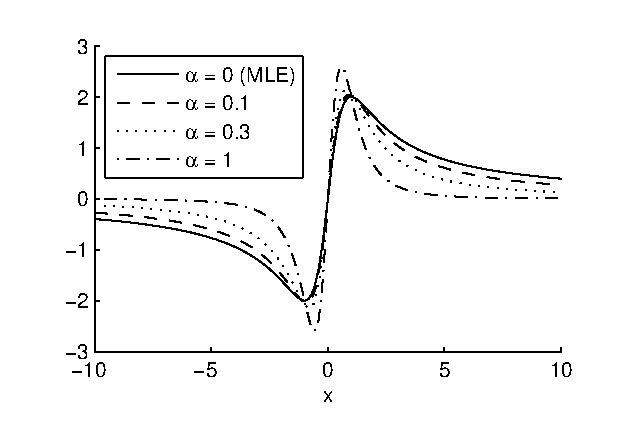
\epsfig{file=Cauchy-IF-mu.eps, height=2.6in} \\
	$\mathrm{IF}(x;T_{\mathfrak{R}_\alpha},\mu = 0) $ při $\sigma = 1$ známém
\end{tabular}
\caption{Influenční funkce {\mRao}ů pro Cauchyovo rozdělení}
\label{fig:cauchy-if}
\end{center}
\end{figure}

\noindent Podle vzorce \eqref{IF} se  nakonec podařilo dopočítat influenční funkci pro odhad měřítka $\theta = \sigma$ při znalosti polohy $\mu$. Následujícího výsledku bylo dosaženo výpočtem ve \texttt{Wolfram Mathematica}. Výsledný tvar je tedy

\begin{eqnarray}
\mathrm{IF}(x;T_{\mathfrak{R}_\alpha},\sigma) &=& -\left[4 \sqrt{\pi } (1+\alpha )^2 \sigma ^{2+\alpha } \left(\frac{\sigma }{(x-\mu )^2+\sigma ^2}\right)^{\alpha} \right. \nonumber\\
&&\left(\frac{1}{\sigma }+\frac{\alpha  \left(\frac{1}{\sigma }\right)^{\alpha } \sigma ^{-1+\alpha }}{1+\alpha }-\frac{2 \sigma }{(x-\mu )^2+\sigma ^2}\right) \left. \cos[\pi  \alpha ] \Gamma[\alpha ] \Gamma[1+\alpha ]  \frac{}{} \right] / \nonumber \\ %prázdný zlomek je tam kvůli roztažení koncové závorky
&&\left(4^{1-\alpha } \sqrt{\pi } \left(\frac{1}{\sigma }\right)^{\alpha } \sigma ^{\alpha } \left(-1+\alpha  \left(-1+\alpha  \left(-2+\left(\frac{1}{\sigma }\right)^{\alpha } \sigma ^{\alpha }\right)\right)\right) \right.\nonumber \\ 
&&\left. \cos[\pi  \alpha ] \Gamma[1+2 \alpha ]+1/(3 (3+4 \alpha  (2+\alpha )))\right. \nonumber \\
&& 8 \pi  (1+\alpha ) \left(-1+\alpha  (1+\alpha )^2\right) \Gamma[\alpha ] \nonumber \\
&& \left(6 (1+\alpha ) ^r_2\mathrm{F}_1\left[\frac{1}{2},2,\frac{1}{2}-\alpha ,1\right]-4^{-\alpha } \Gamma[4+2 \alpha ] \right. \nonumber \\
&& \left. \left. ^r_2\mathrm{F}_1\left[\frac{1}{2}+\alpha ,1+\alpha ,-\frac{1}{2}+\alpha ,1\right]\right)\right),
\end{eqnarray}

\noindent kde $^r_2\mathrm{F}_1[a,b;c;z]$ je regularizovaná hypergeometrická funkce 

\begin{equation}
	^r_2\mathrm{F}_1[a,b;c;z] = {\frac{1}{\Gamma[c]}} {_2\mathrm{F}_1}[a,b;c;z],
\end{equation}
přičemž hypergeometrická funkce je definovaná vztahem
\begin{equation}
	{_2\mathrm{F}_1}[a,b;c;z]=\sum _{n=0}^{\infty } \frac{(a)_n (b)_n z^n}{ (c)_n n!}, \qquad |z|<1, \, \text{ nebo } \, (|z|=1\l  \,\text{a} \,  c>a+b),
\end{equation}

\noindent kde $(a)_n$ je Pochhammerův symbol definovaný

\begin{equation}
(a)_n=\prod _{k=0}^{n-1} (a+k), \qquad n \in \mathbb{N}.
\end{equation}

\noindent Kvůli definici hypergeometrické funkce tato influenční funkce však nemá smysl, protože z definičních podmínek nám vychází $\frac{1}{2}+\alpha  + 1+\alpha < -\frac{1}{2}+\alpha $, tedy $\alpha < -2$, což ale odporuje výběru $\alpha>0$ z věty \ref{renyi-veta}. 

\section{Weibullovo rozdělení} %%%%%%%%%%%%%%%%%%%%%  WEIBULL   %%%%%%%%%%%%%%%%%%%%%%

Posledním zpracovávaným rozdělením, bylo tříparametriké Weibullovo s parametrem $\theta = (\mu,\lambda,k)$ a hustotou pravděpodobnosti
\begin{equation}
	p_\theta =  \frac{k}{\lambda} \left( \frac{x-\mu}{\lambda} \right)^{k-1} \exp \left[ -\left( \frac{x-\mu}{\lambda} \right)^k \right], \qquad \mu \in \mathbb{R}, \, \lambda>0, \, k>0, \, x \geq \mu.
\end{equation}

\noindent Pro $\alpha = 0$ je minimální Rényiho odhad roven

\begin{align}
	\hat{\theta}_{\mathfrak{R}_0,n} & = \arg \max_{\theta \in \Theta} \frac{1}{n} \sum^n_{i=1} \ln \left[ \frac{k}{\lambda} \left( \frac{x_i-\mu}{\lambda} \right)^{k-1} 
	\exp \left[ -\left( \frac{x_i-\mu}{\lambda} \right)^k \right]\right] \nonumber \\
	&=\arg \max_{\theta \in \Theta}\left[ \ln \frac{k}{\lambda} + \frac{k-1}{n} \sum^n_{i=1} \ln \left[  \frac{x_i-\mu}{\lambda} \right] - 
	\frac{1}{n} \sum^n_{i=1} \left(  \frac{x_i-\mu}{\lambda} \right)^k \right].
\end{align}

\noindent Podmínka \ref{beta-podminka} opět platí pro každé $\beta>0$. Pro $\alpha>0$ pak vychází minimální $\mathfrak{R}_\alpha$-odhad \eqref{Renyi-estimator_formula} parametrů ve Weibullově modelu ve tvaru

\begin{eqnarray}
	\hat{\theta}_{\mathfrak{R}_\alpha,n} & = & \arg \max_{\theta \in \Theta} \left( \frac{k}{\lambda} \right)^\frac{\alpha}{1+\alpha} (1+\alpha)^{\frac{\alpha}{1+\alpha}\frac{1+\alpha+k}{k}} 
	\Gamma\left(\frac{1+\alpha+k}{k}\right)^{-\frac{\alpha}{1+\alpha}} \nonumber \\
	&& \frac{1}{n}\sum_{i=1}^n \left( \frac{x_i-\mu}{\lambda}\right)^{\alpha(k-1)} \exp\left[-\alpha \left(\frac{x_i-\mu}{\lambda}\right)^k\right].
\end{eqnarray}

\noindent Kvůli použití $\Gamma$-funkce dostáváme dodatečnou podmínku $1+\alpha+k>0$, tedy $\alpha + k > -1$. Tato podmínka je ale splněna automaticky, protože jsou oba parametry kladné. 

Influenční funkce $\eqref{IF}$ pro odhad polohy $\theta = \mu$ pří známých parametrech $\lambda, k $  má tvar

\begin{equation}
	\mathrm{IF}(x;T_{\mathfrak{R}_\alpha},\mu) = \frac{(1+\alpha )^{\frac{-2-\alpha +k (3+\alpha )}{k}} \lambda \left(1+k \left(-1+\left(\frac{x-\mu }{\lambda }\right)^k\right)\right) 
	 \left(\frac{x-\mu }{\lambda }\right)^{\alpha k-\alpha-1}\exp \left[-\alpha\left(\frac{x-\mu }{\lambda }\right)^k\right]}
	 {(-1+k) (-1+k+k \alpha ) \Gamma\left[\frac{-2+k+(-1+k) \alpha }{k}\right]}.
	\label{IF-weibull-mu}
\end{equation}

\noindent Z použití $\Gamma$-funkce vyplývá podmínka $k > 1 + \frac{1}{1+\alpha}$, tedy $(\forall \alpha> 0) (k > 1)$. Pro $\alpha > 0$ opět kvůli exponenciálnímu členu platí

\begin{equation}
	\lim_{x \rightarrow \pm\infty} \mathrm{IF}(x;T_{\mathfrak{R}_\alpha},\mu) = 0.
\end{equation}

\begin{figure}[!htb]
\begin{center}
\begin{tabular}{cc}
	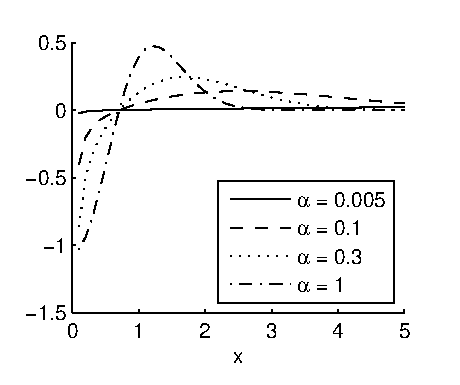
\epsfig{file=Weib-IF-mu.eps, height=2.2in} & 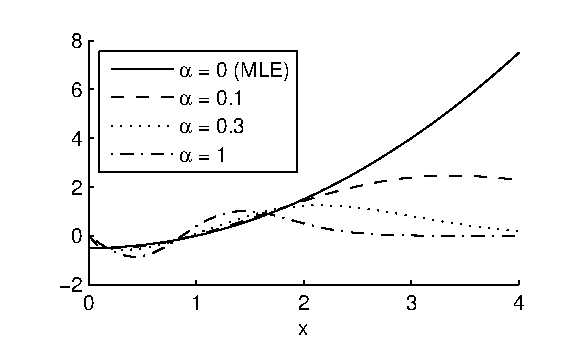
\epsfig{file=Weib-IF-lambda.eps, width=3.2in}
	\\	
	$\mathrm{IF}(x;T_{\mathfrak{R}_\alpha},\mu = 0) $, známé $\lambda = 1, \: k = 2$ & $\mathrm{IF}(x;T_{\mathfrak{R}_\alpha},\lambda = 1) $, známé $\mu = 0, \: k = 2$
\end{tabular}
\caption{Influenční funkce {\mRao}ů $\mu$ a $\lambda$ Weibullovo rozdělení}
\label{figJK:weibull-if}
\end{center}
\end{figure}

\noindent Na obrázku \ref{figJK:weibull-if} je vidět, že je influenční funkce opět omezená. V obrázku není vykreslena funkce pro $\alpha = 0$, protože pro $k=2$ je nutné použít $\alpha >0$.
Pro odhad měřítka $\theta = \lambda$ při známých $\mu, k$ má influenční funkce tvar

\begin{equation}
	\mathrm{IF}(x;T_{\mathfrak{R}_\alpha},\lambda) = \frac{(1+\alpha )^{2+\alpha -\frac{\alpha }{k}} \lambda  \left(\alpha +k (1+\alpha ) \left(-1+\left(\frac{x-\mu }{\lambda }\right)^k\right)\right)
	\left(\frac{x-\mu}{\lambda}\right)^{\alpha k-\alpha} \exp \left[-\alpha\left(\frac{x-\mu}{\lambda}\right)^k\right]}
	{k^2 \Gamma\left[2+\alpha -\frac{\alpha }{k}\right]}.
	\label{IF-weibull-lambda}
\end{equation}

\noindent Opět z použití $\Gamma$-funkce vyplývá $k>\frac{\alpha}{2+\alpha}$. Funkce pro $\alpha > 0$ a $x\rightarrow \pm \infty$ konverguje k $0$ a je omezená. což je vidět i na obrázku \ref{figJK:weibull-if}. Pro odhad parametru $\theta = k$ jsme influenční funkci opět počítali ve \texttt{Wolfram Mathematica}. Funkce vyšla ve tvaru

\begin{eqnarray}
	\mathrm{IF}(x;T_{\mathfrak{R}_\alpha},k)& = &\left(k^2 (1+\alpha )^{2+\alpha -\frac{\alpha }{k}} \left(e^{-\left(\frac{x-\mu }{\lambda }\right)^k} \left(\frac{x-\mu }{\lambda }\right)^{-1+k}\right)^{\alpha } \right. \nonumber \\
	&& \left(\alpha  \text{ln}[1+\alpha ]+k \left(1-k (1+\alpha ) \left(-1+\left(\frac{x-\mu }{\lambda }\right)^k\right)\right.\right. \nonumber \\
	&& \left.\left.\left.\left.\text{ln}\left[\frac{x-\mu }{\lambda }\right]\right)-\alpha  \psi\left[0,1+\alpha -\frac{\alpha }{k}\right]\right)\right)\right/ \nonumber \\
	&& \left(\Gamma\left[1+\alpha -\frac{\alpha }{k}\right] (k (k+\ln[1+\alpha ] \right. \nonumber \\
	&& (-2 k+2 \alpha +(k+(-1+k) \alpha ) \ln[1+\alpha ]))-2 k (-k+\alpha +(k+(-1+k) \alpha ) \nonumber \\
	&& \ln[1+\alpha ]) \psi\left[0,1+\alpha -\frac{\alpha }{k}\right]+k (k+(-1+k) \alpha ) \nonumber \\
	&& \left.\left.\psi\left[0,1+\alpha -\frac{\alpha }{k}\right]^2+\left(k^2+(-1+k) k \alpha +\alpha ^2\right) \psi\left[1,1+\alpha -\frac{\alpha }{k}\right]\right)\right),
	\label{IF-weibull-k}
\end{eqnarray}

\noindent kde $\psi(n,z)$ je $(n+1)-$tá derivace logaritmu $\Gamma(z)$, tedy

\begin{equation}
	\psi(n,z) = \frac{\mathrm{d}^{n+1}}{\mathrm{d}z^{n+1}} \ln \Gamma(z).
\end{equation}

\noindent Kvůli použití $\Gamma$-funkce vzniká podmínka $k > \frac{\alpha}{1+\alpha}$. Funkce je pro $\alpha>0$ opět omezená a pro $x$ rostoucí nade všechny meze konverguje k 0. Na obrázku \ref{figJK:weibull2-if} je patrné, že tento odhad bude fungovat kvůli velké absolutní hodnotě influenční funkce lépe pro větší hodnoty $\alpha$.

\begin{figure}[htb]
\begin{center}
\begin{tabular}{cc}	
	\multicolumn{2}{c}{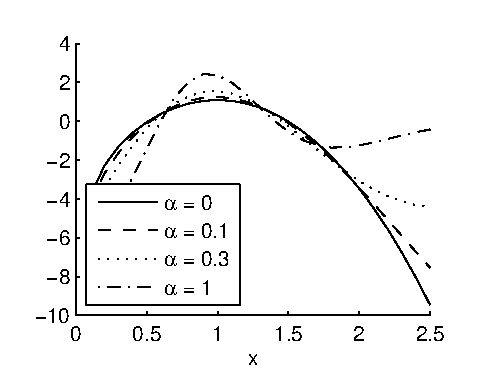
\epsfig{file=Weib-IF-k.eps, height=2.5in}}
	\\
	\multicolumn{2}{c}{$\mathrm{IF}(x;T_{\mathfrak{R}_\alpha},k = 2) $, známé $\mu = 0, \: \lambda = 1$}
\end{tabular}
\caption{Influenční funkce {\mRao}u $k$ pro Weibullovo rozdělení}
\label{figJK:weibull2-if}
\end{center}
\end{figure}



 


